\documentclass[a4paper,12pt,twoside]{article}

\title{FIT 5047: Assignment 1}
\author{Tung X. Nguyen\\
ID 30555418\\
Activity No.31\\
Tutor: Nicholas Spyrison}

\date{\today}

\setcounter{tocdepth}{3}


\usepackage{graphicx}
\graphicspath{ {./img}}

\usepackage{amsmath}
\usepackage{indentfirst}
\usepackage{amssymb}
\usepackage[showframe=false]{geometry}
\usepackage{booktabs}
\usepackage{amsmath}
\usepackage{tabularx}

\usepackage[english]{babel}
\usepackage[utf8]{inputenc}
\usepackage{fancyhdr}
\setlength{\headheight}{15.2pt} 
 
\pagestyle{fancy}
\fancyhf{}
\fancyhead[LE,RO]{Tung X. Nguyen}
\fancyhead[RE,LO]{FIT 5047: Assignment 1}
\fancyfoot[LE,RO]{\thepage}
\fancyfoot[CE,CO]{\leftmark}

\renewcommand{\headrulewidth}{2pt}
\renewcommand{\footrulewidth}{1pt}

\begin{document}
\maketitle


\thispagestyle{empty}

\tableofcontents
\thispagestyle{empty}
\newpage

\oddsidemargin = 22pt
\evensidemargin = 22pt
\marginparsep = 10pt
\marginparwidth = 35pt


\section{Data Wrangling.}
The raw data is read directly into Tableau with the "Data Interpreter" options. Next, columns with numeric values of bleaching percentages are pivotted so that the result contain only one column telling this attribute. Finally, new fields "Coral types" and "Year" are created using the "Create calculating fields" functionality. Here is an image of how the data looks like after wrangling:
\begin{figure}[h]
\caption{Data after wrangling}
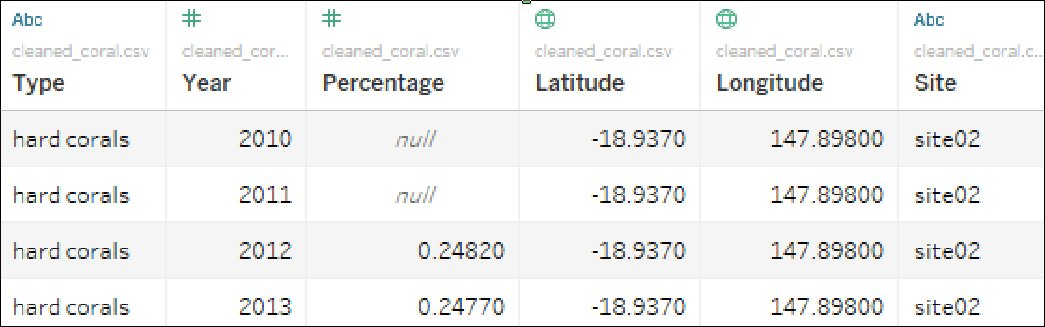
\includegraphics[scale=.4]{img/wr.jpg}
\centering
\end{figure}
\section{Data Exploration.}

\subsection*{Error 1: The percentage in some entries}
\addcontentsline{toc}{subsection}{Error 2: The percentage in some entries}
To discover anomalies in the data, I plot all the percentage data as in Figure 2. Each line shows the trend corresponding to each type of corals throughout the years. There are two questionable data points that could be spotted from this figure:

\begin{figure}[h]
\caption{Line plot for the whole data}
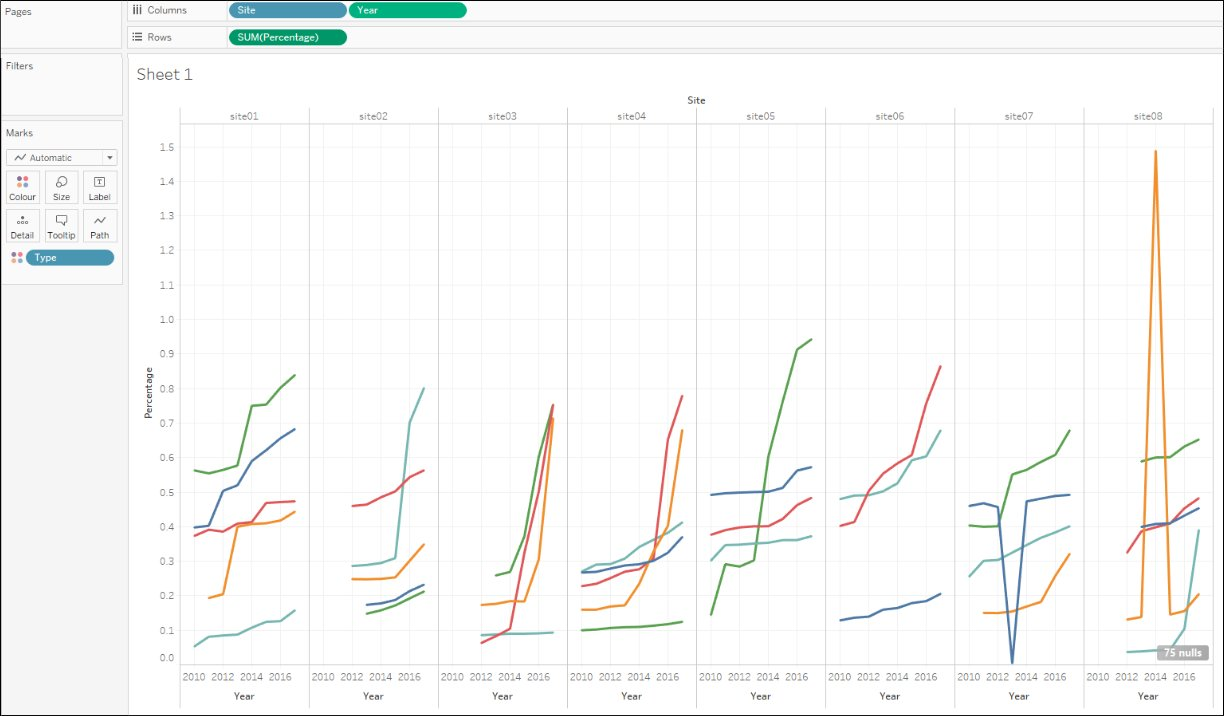
\includegraphics[width=14.5cm]{img/e2.jpg}
\end{figure}
\begin{figure}[!]
\caption{Line plot for the whole data (corrected)}
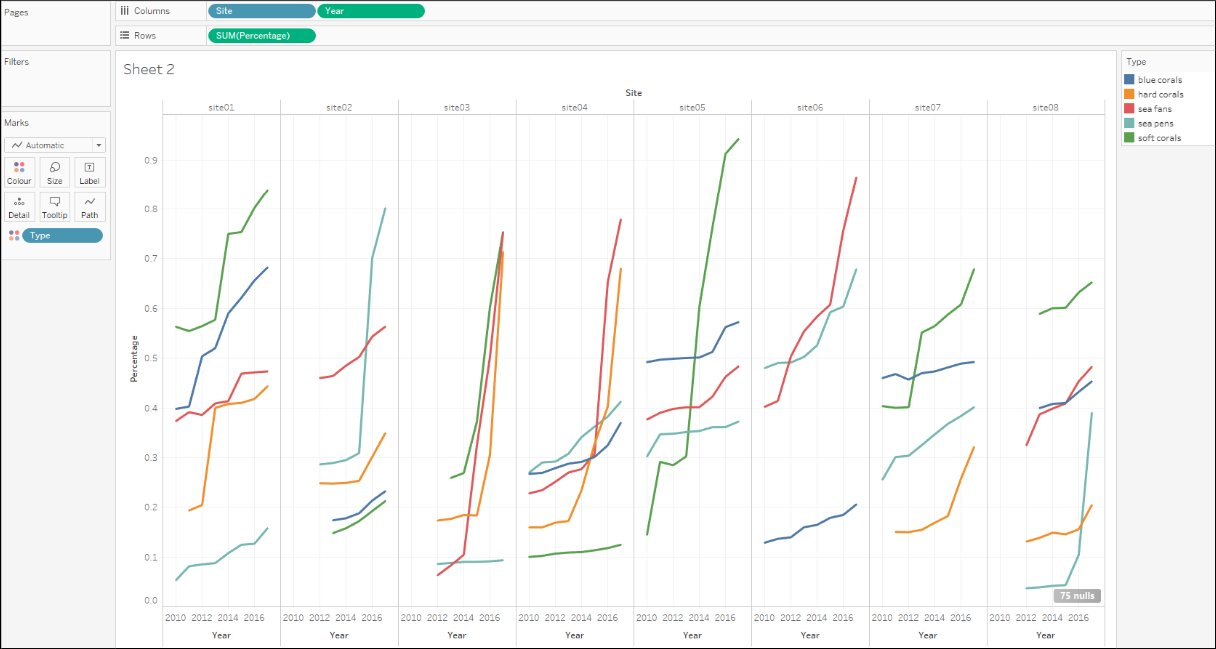
\includegraphics[width=14.5cm]{img/e22.jpg}
\end{figure}

\begin{itemize}
\item Blue corals, Site 7, year 2013: The percentage is unusually low (nearly 0\%), compared to other data points
\item Hard corals, Site 8, year 2014: The number is bigger than 1, which is apparently incorrect.
\end{itemize}

My explanation for these anomalies is simply human error: extra or missed digits because of typos. My solution is to adjust the decimal points so that the trend is smoothed out. The final result should look like Figure 3.


\subsection*{Error 2: The location of site 2}
\addcontentsline{toc}{subsection}{Error 1: The location of site 2}
Tthe location of all sites is shown in Figure 4. It is obvious that the location of site 2 is off the Great Barrier Reef. After looking at the data, I conclude that the latitude of site 2 should be negative, not positive as recorded. To fix this, I exported the wrangled data to a csv file, then make a copy of this file and fix the sign of the latitude on this copy using Excel.
\begin{figure}[h]
\caption{Site 2 with wrong location}
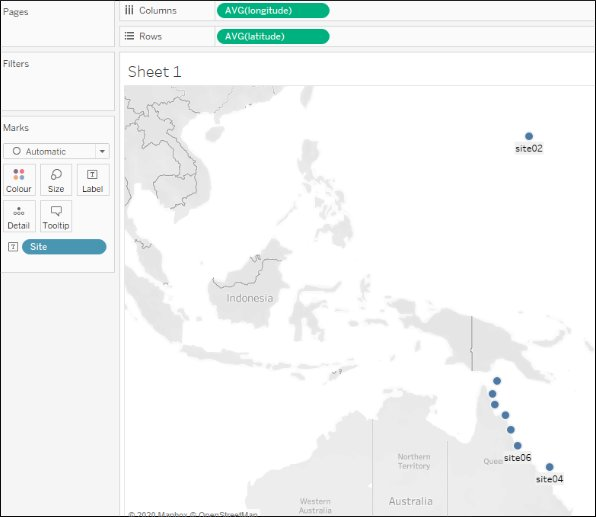
\includegraphics[scale=0.5]{img/e1.jpg}
\centering
\end{figure}

\begin{figure}[h]
\caption{Location with corrected cordinates}
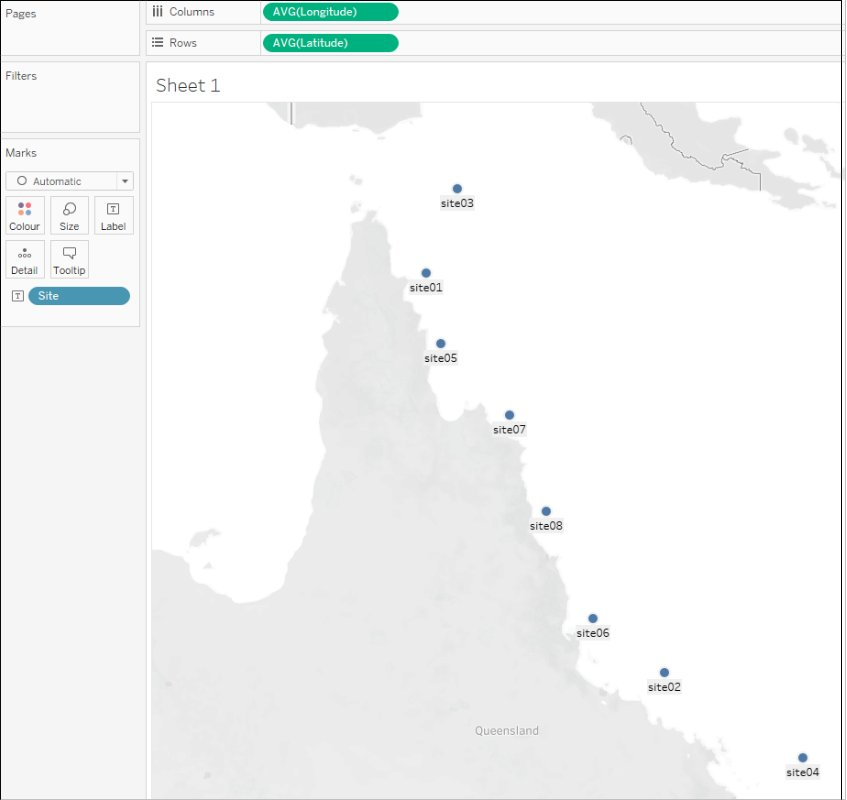
\includegraphics[scale=0.35]{img/e11.jpg}
\centering
\end{figure}

After fixing this error, the result is shown in Figure 5


\section{Answering Questions.}
\subsection*{Q1}
\addcontentsline{toc}{subsection}{Q1}
Looking at Figure 3, I conclude that the bleaching effect is the worst for soft corals in site 5, year 2017 with the recorded number is 94.23\%.
\subsection*{Q2}
\addcontentsline{toc}{subsection}{Q2}
The bleaching of blue corals was the worst in site 1, which started at averagely high (40\%) compared to other sites, then quickly rose to the highest in 2017 (nearly 70\%). Overall, blue corals were being bleached in all sites and the numbers were consistently increasing. However, it is clear that sites that are closer to the North (sites 1, 5 and 7) had higher bleaching percentages for blue corals than other sites.

The same trend was seen in the bleaching of soft corals. Southern sites (site 2, 4) had the lowest and most stable bleaching percentage, while the number for Northern ones skyrocketed over the years.

For hard corals, all sites started with small differences, but site 3 and site 4 finished the period with the highest numbers, respectively 71\% and 68\%. It seems that the sites at the center of the reef (site 7, 8) had less severe bleaching effects on hard corals.

For sea fans, by the end of the period, sites 3, 4, and 6  held the highest percentages, all above 70\%. It is worth noticing that site 3, which is the furthest to the North, started out with the smallest number (6\%) but quickly rose to the top over the years.

Sea pens were more bleached in Southern sites of the reef (site 2, 6, 4), compared to the rest. Specifically, the highest number was above 70\% for site 2, and the smallest percentage was under 1\% for site 3. The situation was not too serious for site 2 until 2015 when this site showed a remarkable gain in the bleaching percentage.



\end{document}